\documentclass{standalone}
\usepackage{tikz}

\begin{document}
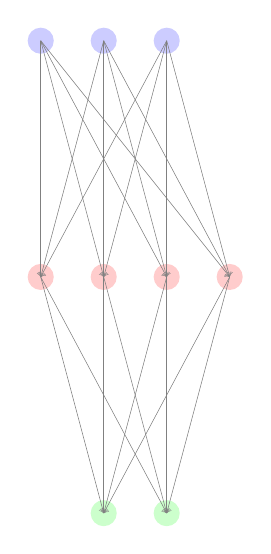
\begin{tikzpicture}[x=1cm,y=1cm]
    % Define layers
    \def\nodespacing{0.8} % spacing between nodes
    \def\layersep{3}     % separation between layers
    
    % Draw input layer (3 nodes)
    \foreach \i in {1,...,3} {
        \node[circle,fill=blue!20] at (\nodespacing*\i-\nodespacing*2,\layersep) {};
    }
    
    % Draw hidden layer (4 nodes)
    \foreach \i in {1,...,4} {
        \node[circle,fill=red!20] at (\nodespacing*\i-\nodespacing*2,0) {};
    }
    
    % Draw output layer (2 nodes)
    \foreach \i in {1,...,2} {
        \node[circle,fill=green!20] at (\nodespacing*\i-\nodespacing, -\layersep) {};
    }
    
    % Draw connections from input to hidden layer
    \foreach \i in {1,...,3} {
        \foreach \j in {1,...,4} {
            \draw[->, very thin, color=gray] (\nodespacing*\i-\nodespacing*2,\layersep) -- (\nodespacing*\j-\nodespacing*2,0);
        }
    }
    
    % Draw connections from hidden to output layer
    \foreach \i in {1,...,4} {
        \foreach \j in {1,...,2} {
            \draw[->, very thin, color=gray] (\nodespacing*\i-\nodespacing*2,0) -- (\nodespacing*\j-\nodespacing,-\layersep);
        }
    }
\end{tikzpicture}
\end{document}